\documentclass[10pt,a4paper]{article}
\begin{filecontents*}[overwrite]{refs.bib}
@book{kleinberg2006,
  author = {Jon Kleinberg and {\'E}va Tardos},
  title = {Algorithm Design},
  publisher = {Pearson/Addison-Wesley},
  year = {2006}
}
@article{karatsuba1962,
  author = {Anatolii Karatsuba and Yuri Ofman},
  title = {Multiplication of Multidigit Numbers on Automata},
  journal = {Doklady Akademii Nauk SSSR},
  volume = {145},
  number = {2},
  pages = {293--294},
  year = {1962}
}
@inproceedings{shamos1975,
  author = {Michael Ian Shamos and Dan Hoey},
  title = {Closest-Point Problems},
  booktitle = {16th Annual Symposium on Foundations of Computer Science},
  pages = {151--162},
  year = {1975}
}
@book{clrs2022,
  author = {Thomas H. Cormen and Charles E. Leiserson and Ronald L. Rivest and Clifford Stein},
  title = {Introduction to Algorithms},
  edition = {4},
  publisher = {MIT Press},
  year = {2022}
}
@misc{fastapi,
  author = {Sebasti{\'a}n Ram{\'i}rez},
  title = {{FastAPI} Documentation},
  howpublished = {\url{https://fastapi.tiangolo.com}},
  year = {2024}
}
\end{filecontents*}
\usepackage[margin=0.7in]{geometry}
\usepackage{times}
\usepackage{amsmath,booktabs,graphicx,tikz,xcolor,url,array}
\usetikzlibrary{arrows.meta,positioning}
\usepackage[labelfont=bf,font=small]{caption}
\usepackage{titlesec}
\titlespacing*{\section}{0pt}{6pt}{3pt}
\titleformat{\section}{\large\bfseries}{\thesection.}{0.5em}{}
\usepackage{enumitem}\setlist{nosep,leftmargin=1.2em}
\setlength{\parskip}{2pt}
\newcommand{\tbd}{\textcolor{red}{\textbf{TBD}}}
\title{\textbf{\Large Divide-and-Conquer in Practice: Closest Pair of Points and Karatsuba Multiplication with an Interactive Visualizer}}
\author{Ahmed Raza (24K-1010), Simal Hassan (24K-0688), Laiba Jamil (24K-0812)\\ Design and Analysis of Algorithms -- Course Project}
\date{}
\makeatletter\renewcommand{\maketitle}{\par\begingroup\centering{\LARGE\@title\par}\vskip 6pt{\large\@author\par}\vskip 4pt\endgroup}\makeatother
\begin{document}
\maketitle

\section*{Abstract}
We implement two classic divide-and-conquer algorithms in Python: the $O(n\log n)$ closest pair of points in the plane and Karatsuba's integer multiplication, which runs in $O(n^{\log_2 3})\approx O(n^{1.585})$. A seeded generator produces 20 benchmark inputs, from 101 points or digits up to $10^6$, including adversarial cases such as duplicates, collinear points, tied grids and all-9 operands. The algorithms are exposed through a FastAPI backend and a web interface that shows small inputs step by step and large inputs as a final result with running time. Outputs were checked against reference results, and the full benchmark finished on all 20 files, including the $10^6$-point and $10^6$-digit cases.

\section{Introduction}
Divide and conquer splits a problem into smaller independent subproblems, solves them recursively and combines the results. Two textbook cases show how the combine step decides the cost. For closest pair, a brute-force search needs $\Theta(n^2)$ distance checks, but a clever merge brings this to $O(n\log n)$ \cite{shamos1975,kleinberg2006}. For multiplication, the schoolbook method costs $\Theta(n^2)$ digit operations, while Karatsuba reduces four half-size products to three \cite{karatsuba1962}. Our goals are to (i) implement both algorithms correctly, (ii) test them on 10 inputs each that cover typical and degenerate cases, and (iii) build a clear interface that makes the recursion visible.

\section{Proposed System}
Figure~\ref{fig:sys} shows the architecture. The generator writes the datasets; the FastAPI backend \cite{fastapi} reads a selected file and calls \texttt{algorithms.py}; the React front end renders either the step trace or the final result. \texttt{run\_all.py} runs both algorithms on all files for the benchmark table.

\begin{figure}[h]
\centering
\resizebox{\textwidth}{!}{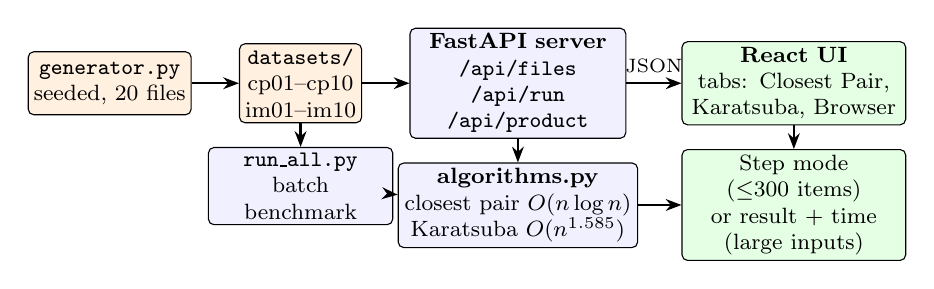
\begin{tikzpicture}[
  node distance=3mm and 6mm,
  box/.style={draw, rounded corners=2pt, align=center, font=\footnotesize, minimum height=8mm, inner sep=2pt, fill=blue!6},
  data/.style={box, fill=orange!12},
  ui/.style={box, fill=green!10},
  arr/.style={-{Stealth[length=2mm]}, thick}]
\node[data] (gen) {\texttt{generator.py}\\seeded, 20 files};
\node[data, right=of gen] (ds) {\texttt{datasets/}\\cp01--cp10\\im01--im10};
\node[box, right=of ds, text width=2.6cm] (api) {\textbf{FastAPI server}\\\texttt{/api/files}\\\texttt{/api/run}\\\texttt{/api/product}};
\node[box, below=of api, text width=2.9cm] (alg) {\textbf{algorithms.py}\\closest pair $O(n\log n)$\\Karatsuba $O(n^{1.585})$};
\node[ui, right=7mm of api, text width=2.7cm] (ui) {\textbf{React UI}\\tabs: Closest Pair,\\Karatsuba, Browser};
\node[ui, below=of ui, text width=2.7cm] (out) {Step mode ($\le$300 items)\\or result + time\\(large inputs)};
\node[box, below=of ds, text width=2.2cm] (run) {\texttt{run\_all.py}\\batch benchmark};
\draw[arr] (gen) -- (ds);
\draw[arr] (ds) -- (api);
\draw[arr] (api) -- (alg);
\draw[arr] (alg.east) -| ([xshift=-3mm]out.west) -- (out.west);
\draw[arr] (api) -- node[above, font=\scriptsize]{JSON} (ui);
\draw[arr] (ui) -- (out);
\draw[arr] (ds) -- (run);
\draw[arr] (run) -- (alg);
\end{tikzpicture}}
\caption{System architecture: data generation, algorithm backend, and visualization front end.}\label{fig:sys}
\end{figure}

\textbf{Closest pair.} Points are sorted by $x$. The set is split at the median $x$-coordinate into $L$ and $R$, and both halves are solved recursively, giving $\delta=\min(\delta_L,\delta_R)$. Only points within $\delta$ of the dividing line can form a closer cross pair. These are scanned in $y$-order, and each point needs to be compared with only a constant number of successors (at most 7) \cite{kleinberg2006}. The points are kept pre-sorted by $y$ through the recursion (merge step), so the combine cost is $O(n)$ and
\begin{equation}
T(n)=2T(n/2)+O(n)\;\Rightarrow\;T(n)=O(n\log n).
\end{equation}
The program returns the pair and the distance. Duplicates give distance 0.

\textbf{Karatsuba.} For $x=x_h10^m+x_l$ and $y=y_h10^m+y_l$, we compute $z_2=x_hy_h$, $z_0=x_ly_l$ and $z_1=(x_h+x_l)(y_h+y_l)-z_2-z_0$, so that
\begin{equation}
xy=z_2\,10^{2m}+z_1\,10^{m}+z_0,\qquad T(n)=3T(n/2)+O(n)=O(n^{\log_2 3}).
\end{equation}
Below a cutoff the code switches to schoolbook multiplication. The cutoff is 20 digits in step mode, so the recursion tree stays visible, and 64 digits for large inputs, for speed.

\textbf{Interface.} Three tabs are provided: \emph{Closest Pair}, \emph{Karatsuba} and \emph{Browser} (lists all dataset files). Files with at most 300 points or digits (cp10, im10) run in step mode with Play/Next controls, a canvas showing splits and the strip, and a recursion tree that shows the $z_0,z_1,z_2$ values and the combine step. Larger files show the answer and the algorithm running time (file reading excluded).

\section{Experimental Setup}
All 20 files are produced by \texttt{generator.py} using a pseudo-random generator seeded per file: cp01--cp10 use seeds 1001--1010 and im01--im10 use seeds 2001--2010 (also stored in \texttt{datasets/seeds.txt}), so every file can be regenerated exactly. Closest-pair files start with $n$ followed by one ``\texttt{x y}'' line per point; multiplication files hold two decimal numbers on two lines. Experiments ran in Python on a laptop with an intel Core i5-10310U CPU(1.70GHz) , 8 GB RAM (7965 MB reported) ,Windows 10(build 19045) and Python 3.15.2. 

\begin{table}[h]
\centering\small
\caption{Input datasets.}\label{tab:data}
\begin{tabular}{@{}l r p{9.6cm}@{}}
\toprule
File & Size & Content and generation method\\
\midrule
cp01--cp04 & $10^3,10^4,10^5,10^6$ & Uniform random real $x,y\in[0,10^6]$\\
cp05 & $10^6$ & Clustered around 10 random centers\\
cp06 & $10^6$ & Integer coordinates in a small range, so many duplicates (distance 0)\\
cp07 & $10^5$ & All points on one vertical line\\
cp08 & $10^5$ & Equally spaced grid, many tied closest pairs\\
cp09 & $10^6$ & Random points with the closest pair placed across the middle dividing line\\
cp10 & 101 & Small file for step-by-step demonstration\\
\midrule
im01--im04 & $10^3,10^4,10^5,10^6$ digits & Random digits, no leading zero\\
im05 & $10^6$ and 10 digits & Operands of very different lengths\\
im06 & $10^5$ digits & One operand is all 9s\\
im07 & 99{,}999 digits & Odd length with many zeros\\
im08 & $10^6$ digits & Both operands are powers of 10\\
im09 & 1 and $10^6$ digits & One operand is 0\\
im10 & 101 digits & Small file for step-by-step demonstration\\
\bottomrule
\end{tabular}
\end{table}

\section{Results and Discussion}
Table~\ref{tab:res} lists the output of \texttt{run\_all.py} (algorithm time only, file reading excluded). All 20 runs finished, including the $10^6$-digit multiplications, so the 100{,}000-digit limit allowed for Python was \emph{not} used. The closest-pair results agree with how each file was constructed (cp06 and cp07 give 0, cp08 gives the grid spacing 10, cp09 gives the planted cross-line pair), and the product digit counts agree with the operand lengths; the im10 product was additionally compared with Python's built-in \texttt{x*y} in our backend tests.

\begin{table}[h]
\centering\small
\caption{Benchmark results from \texttt{python run\_all.py}.}\label{tab:res}
\begin{tabular}{@{}l r r r | l r r r@{}}
\toprule
File & $n$ & Distance & Time (s) & File & Digits & Product digits & Time (s)\\
\midrule
cp01 & $10^3$ & 1052.4329 & 0.01 & im01 & $10^3$ & 1999 & $<$0.01\\
cp02 & $10^4$ & 97.217606 & 0.31 & im02 & $10^4$ & 19999 & 0.06\\
cp03 & $10^5$ & 8.495362 & 4.02 & im03 & $10^5$ & 200000 & 2.58\\
cp04 & $10^6$ & 0.587571 & 60.26 & im04 & $10^6$ & 2000000 & 124.52\\
cp05 & $10^6$ & 0.023398 & 64.14 & im05 & $10^6$/10 & 1000010 & 14.40\\
cp06 & $10^6$ & 0 & 28.46 & im06 & $10^5$ & 200000 & 3.88\\
cp07 & $10^5$ & 0 & 9.55 & im07 & 99{,}999 & 199998 & 3.47\\
cp08 & $10^5$ & 10 & 5.52 & im08 & $10^6$ & 1999999 & 16.82\\
cp09 & $10^6$ & 0.001 & 74.94 & im09 & 1/$10^6$ & 1 (product 0) & 2.26\\
cp10 & 101 & 0.563906 & $<$0.01 & im10 & 101 & 202 & $<$0.01\\
\bottomrule
\end{tabular}
\end{table}

\textbf{Discussion.} For uniform random points (cp01--cp04) each tenfold increase in $n$ multiplies the time by roughly 13--15, slightly above linear, consistent with $O(n\log n)$. For Karatsuba on random inputs (im02--im04) the time grows by a factor of about 40--50 per tenfold increase in digits, close to the predicted $10^{1.585}\approx 38$. Inputs with structure are cheaper: cp06 (28.5\,s) is faster than the random $10^6$-point files because duplicates keep $\delta$ at 0, which empties the strip; im05, im08 and im09 are far faster than im04 because of unbalanced operands, many zeros and a zero operand. cp07 reports 0, so at least two points on the line coincide. cp08 reports 10 with ties broken arbitrarily. cp09 returns 0.001, the planted pair, which is only found in the strip step because the two points lie on opposite sides of the dividing line. Even im09, whose product is 0, takes about 2\,s, which we attribute to handling the $10^6$-digit operand. Absolute times are those of pure Python on our machine and are larger than a compiled implementation would give. For im10, the trace in Figure~\ref{fig:shots}(c) shows the 101-digit input splitting at $m=50$, then 25, then 13, where operands of at most 20 digits fall to the schoolbook base case; the third product $(x_h+x_l)(y_h+y_l)$ gives $z_1$ by subtraction in the COMBINE row.

\begin{figure}[t]
\centering
\begin{tabular}{@{}cc@{}}
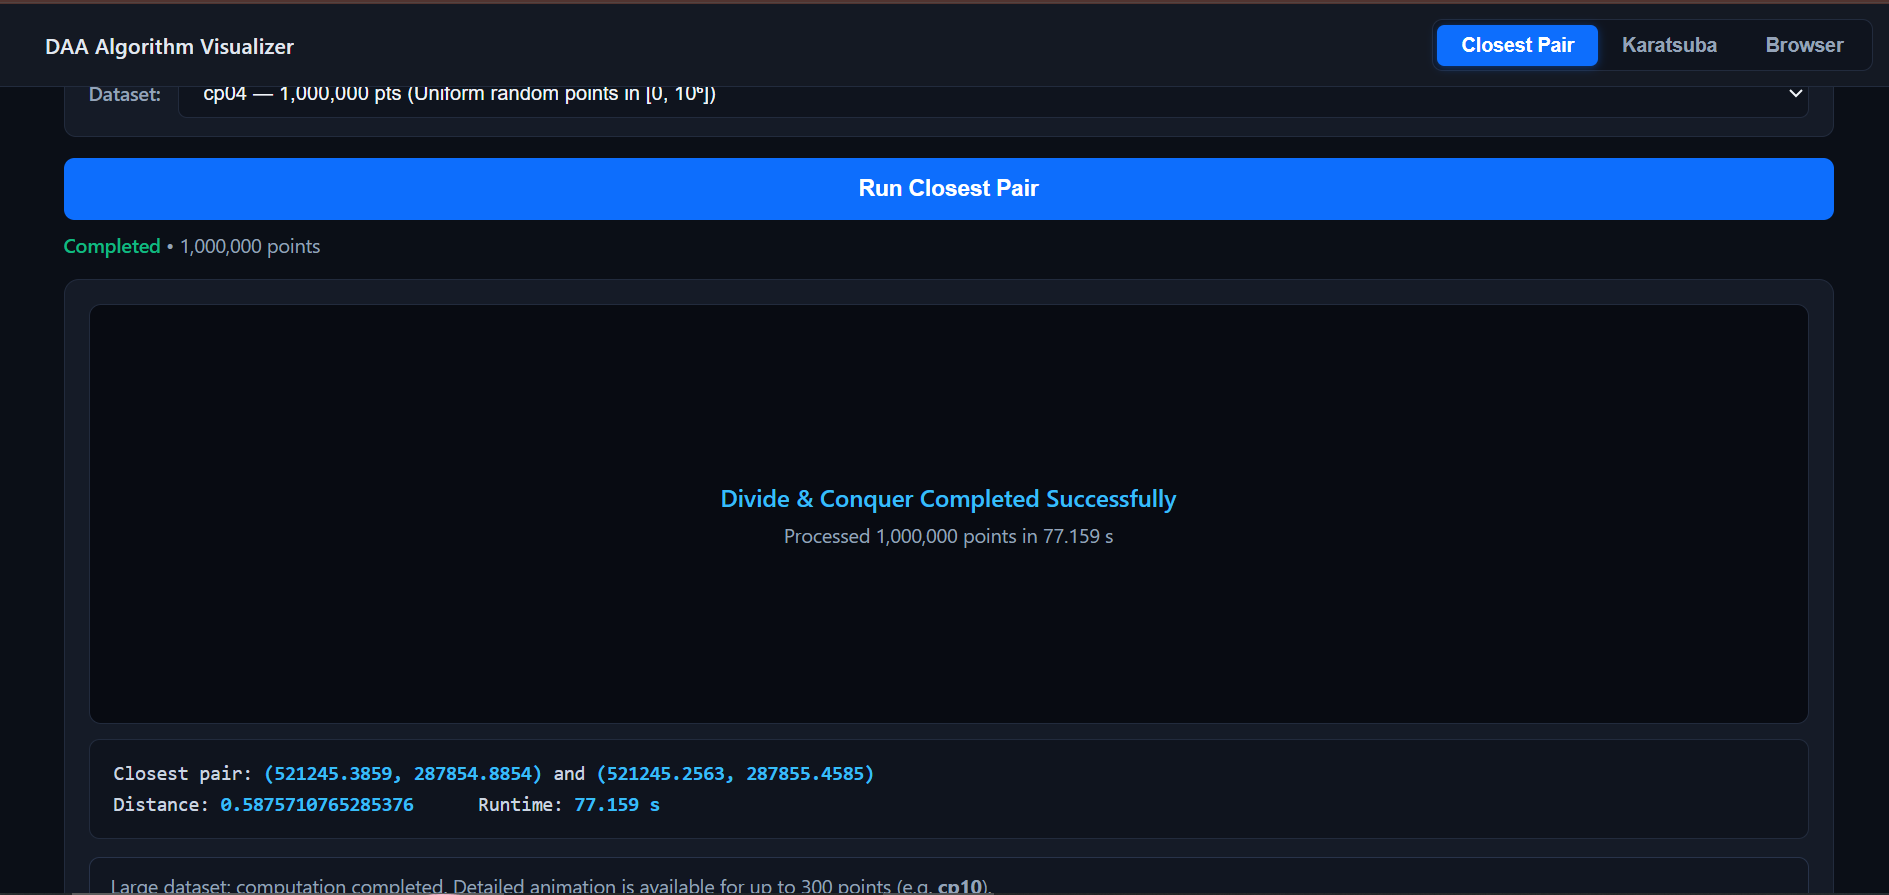
\includegraphics[width=0.485\textwidth]{figures/s1.png} & 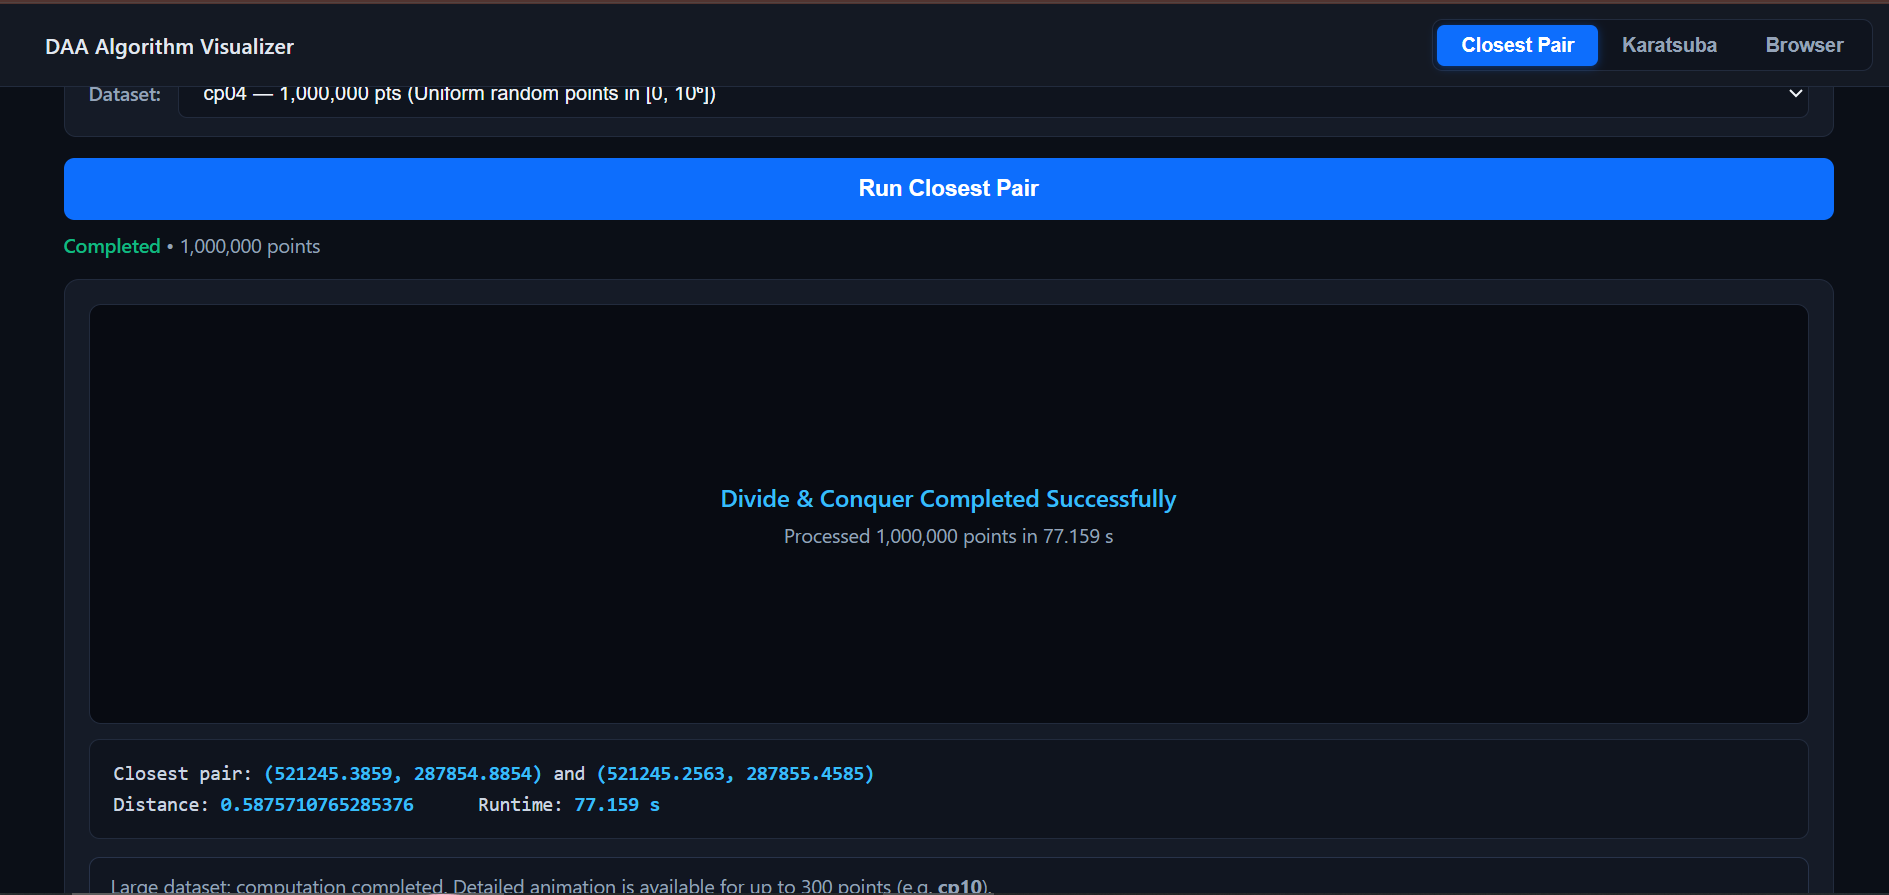
\includegraphics[width=0.485\textwidth]{figures/s7.png} \\
\footnotesize (a) Closest Pair of Points Algorithm Interface using Divide and Conquer & \footnotesize (b) cp04: 1,000,000 points, showing the closest pair, minimum distance, and execution time\\

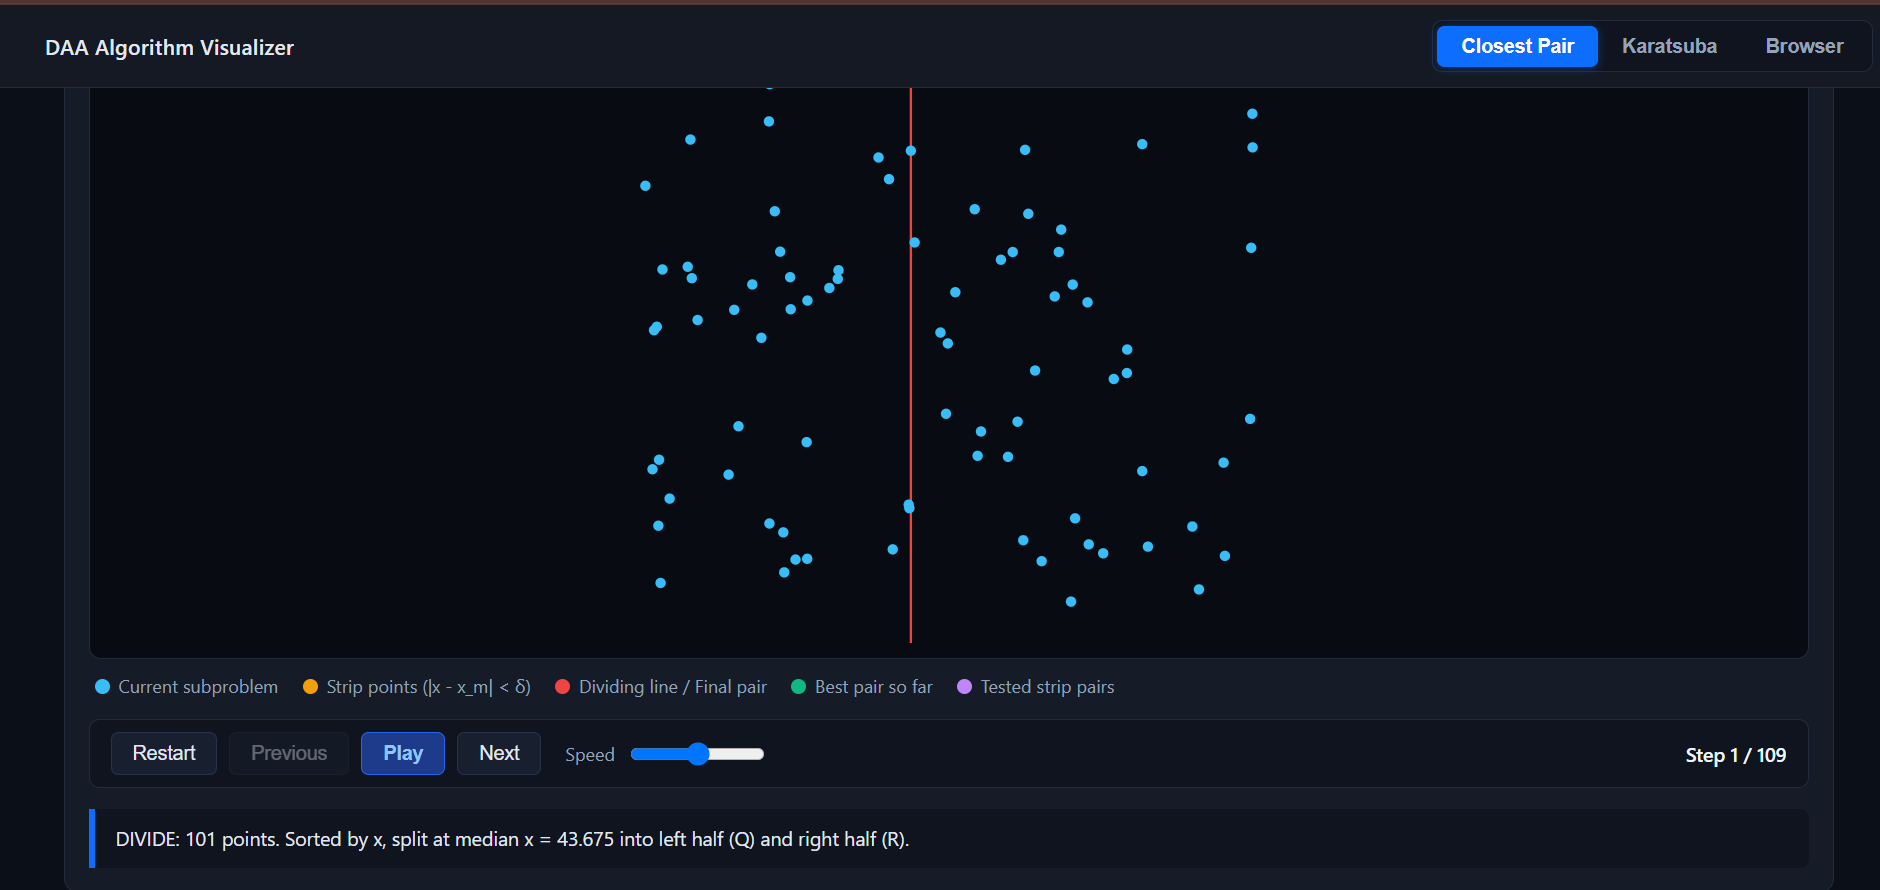
\includegraphics[width=0.485\textwidth]{figures/s2.png} & 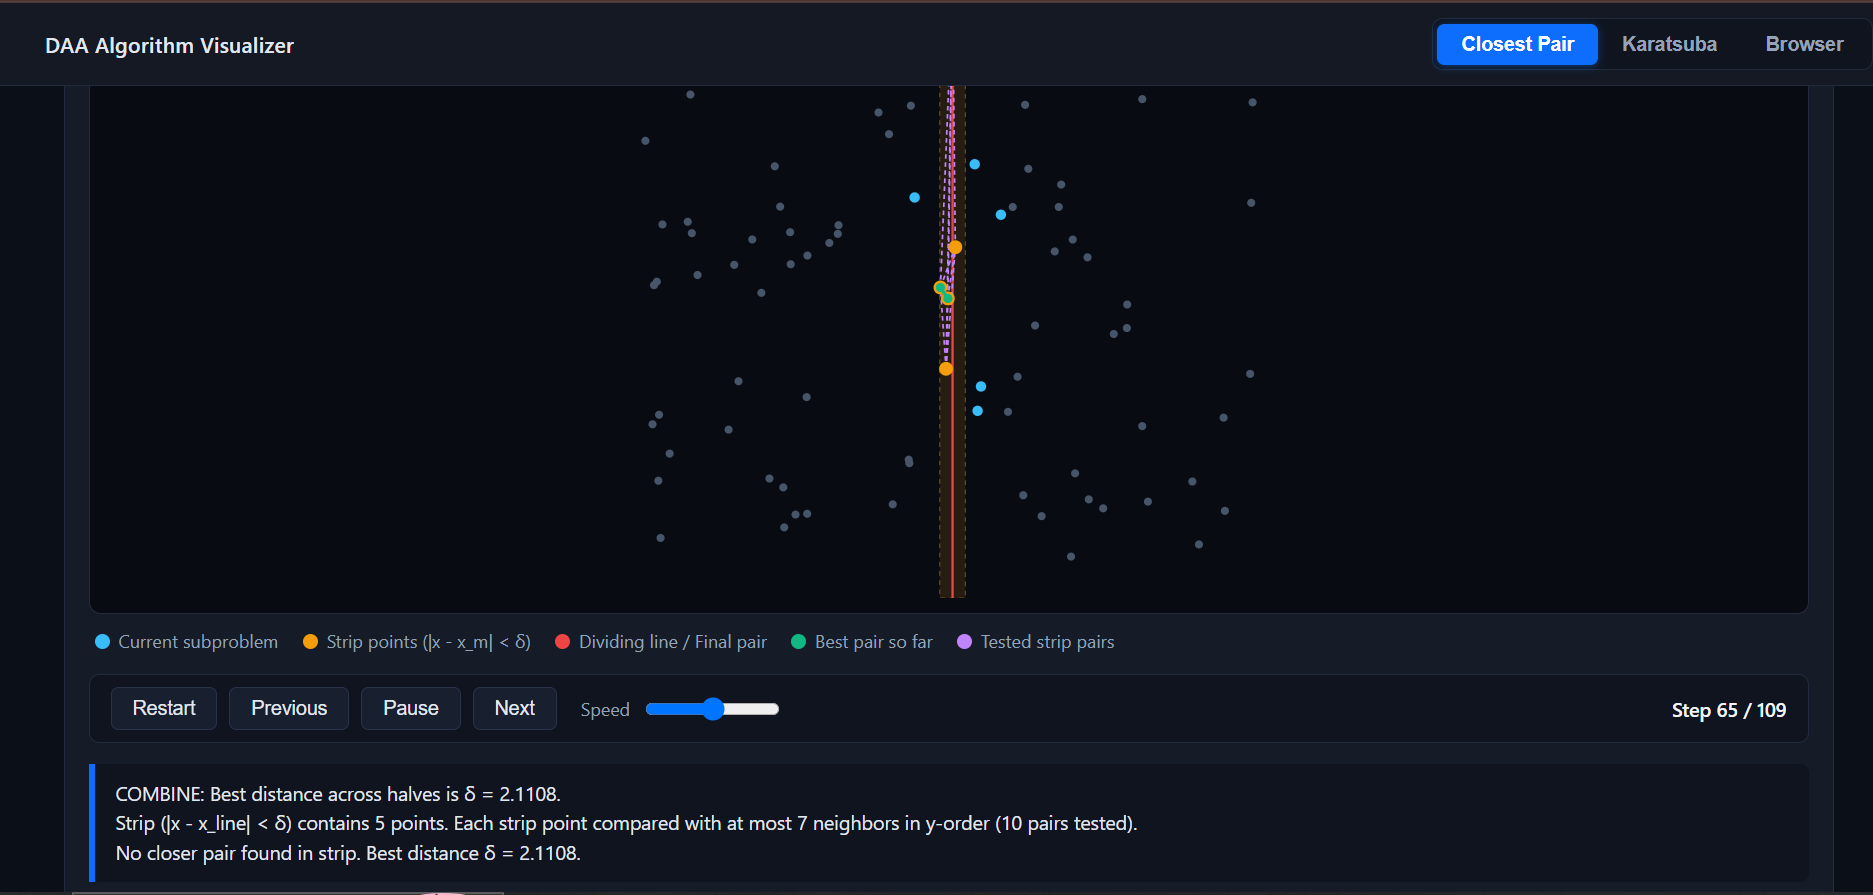
\includegraphics[width=0.485\textwidth]{figures/s3.png}\\
\footnotesize (c) cp10, step 1: divide at the median & \footnotesize (d) cp10, step 65: strip check, $\delta=2.1108$\\[3pt]
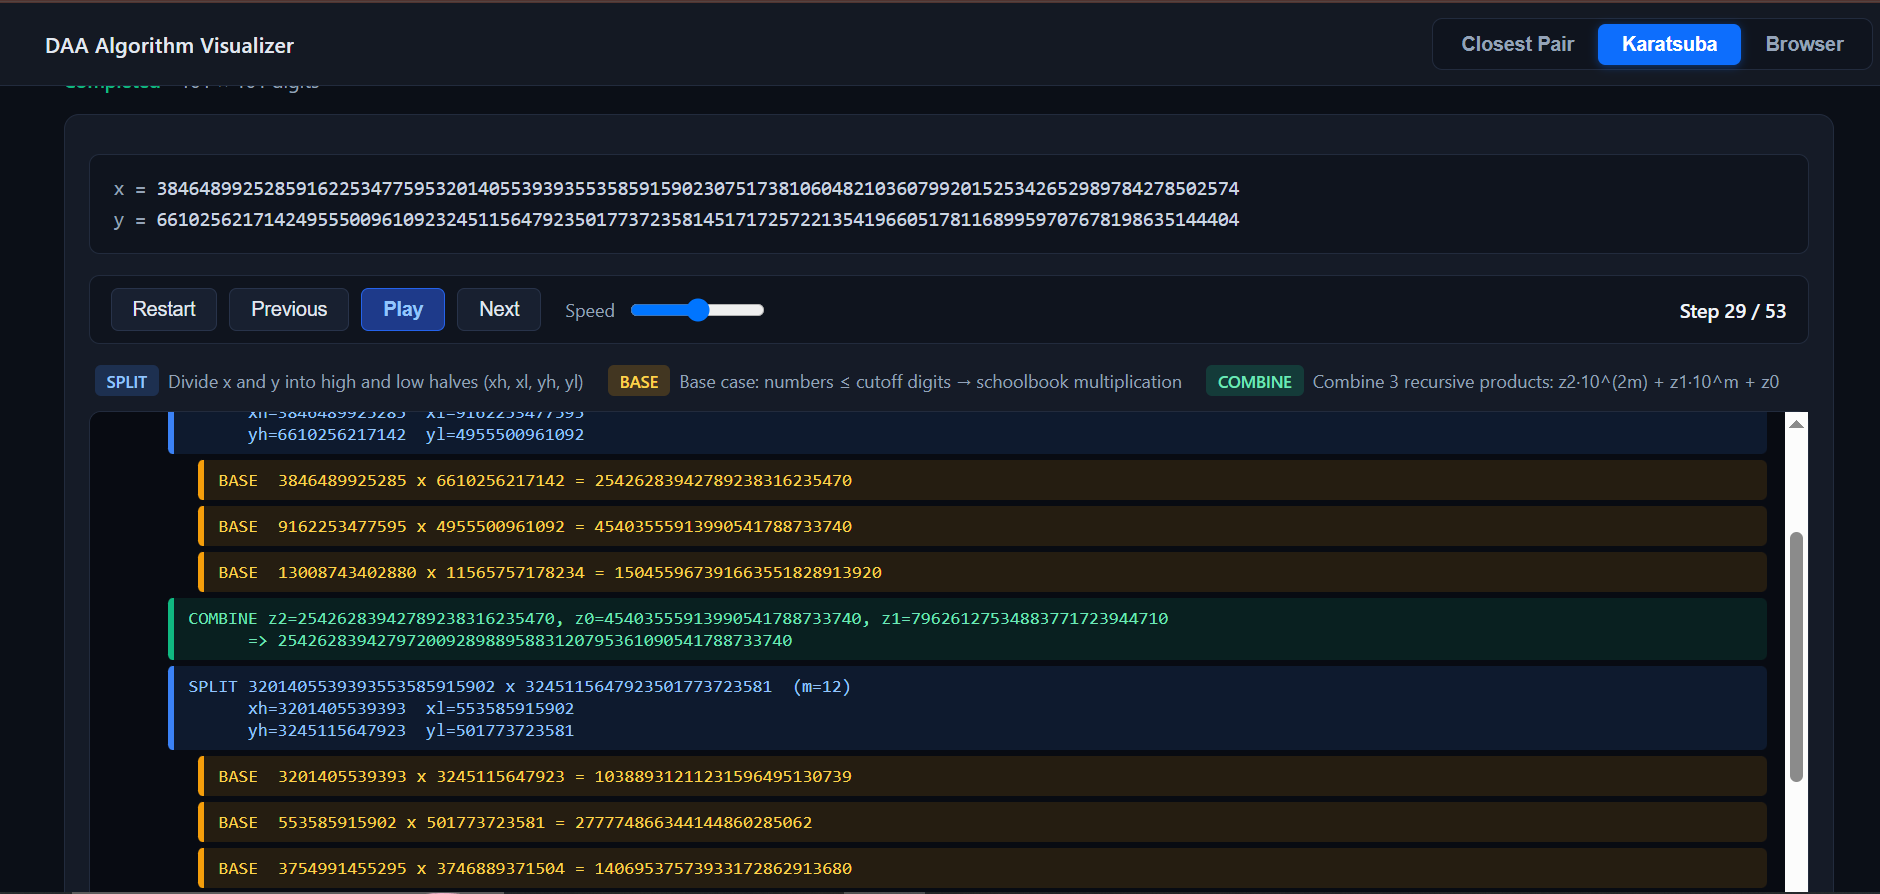
\includegraphics[width=0.485\textwidth]{figures/s4.png} & 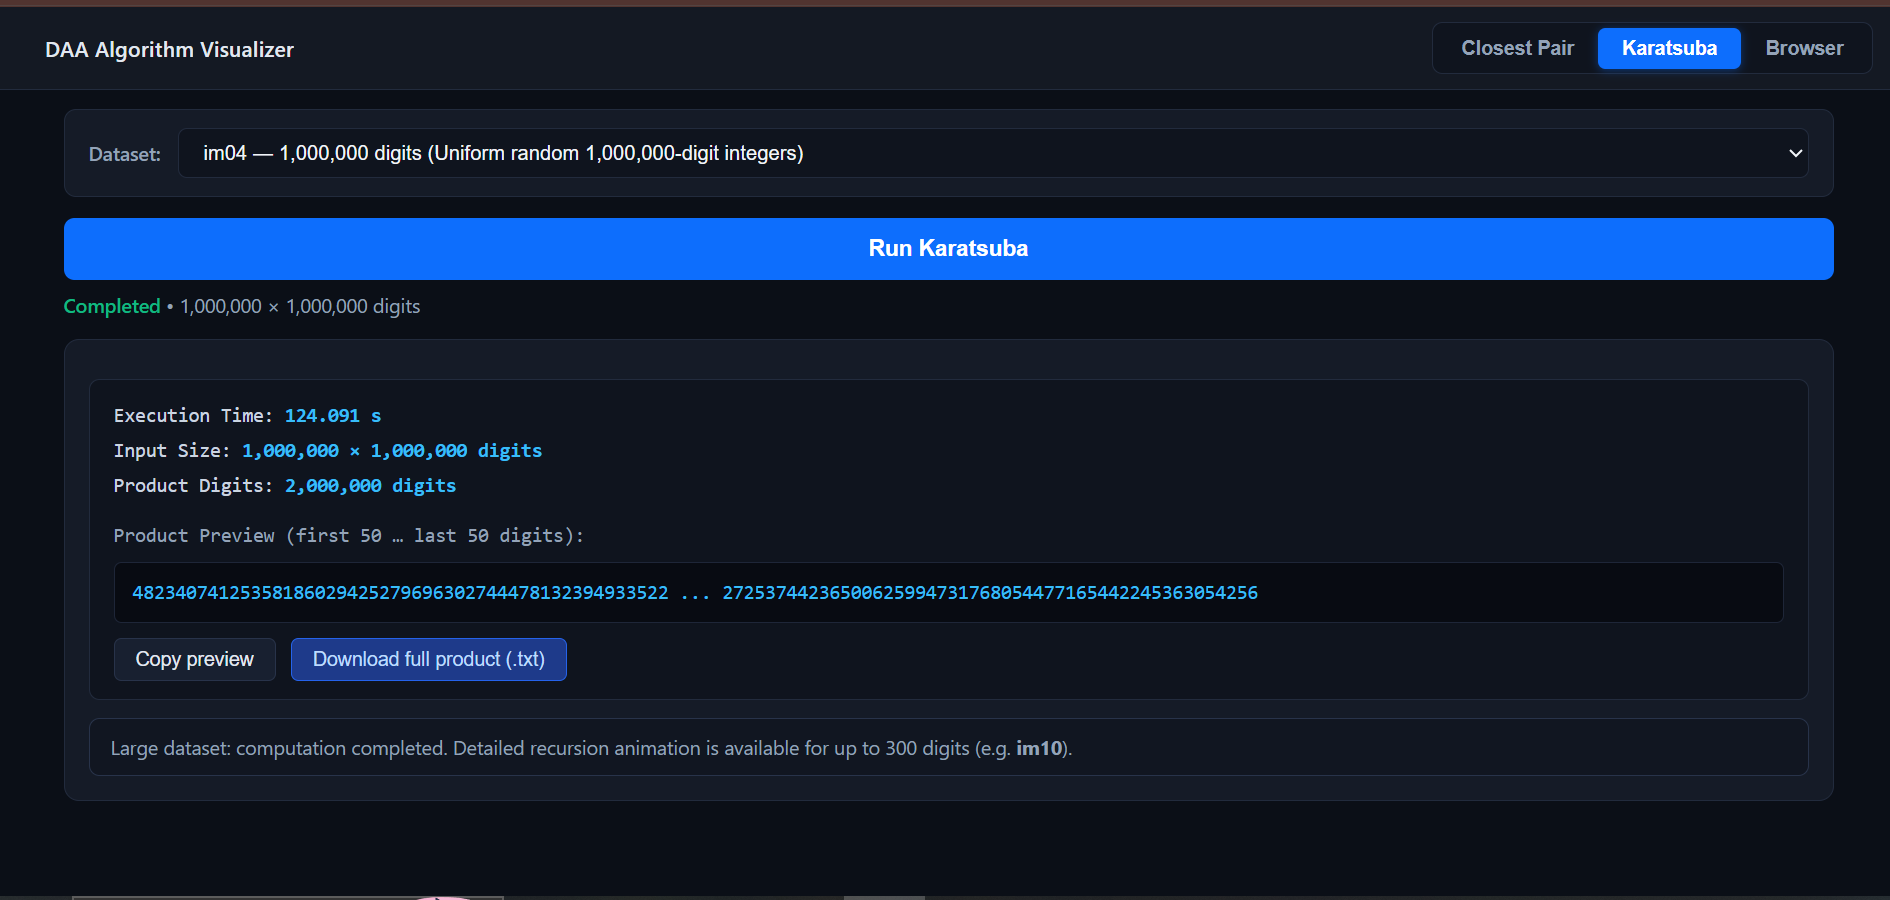
\includegraphics[width=0.485\textwidth]{figures/s6.png}\\
\footnotesize (e) im10, step 29: split, BASE and COMBINE rows & \footnotesize (f) im04: $10^6\times10^6$ digits, result and time\\

\end{tabular}
\caption{User interface in step mode (c)--(e) and on a large input (b),(f).}\label{fig:shots}
\end{figure}

\section{Conclusion}
We implemented and verified both divide-and-conquer algorithms on 20 inputs up to $10^6$ points or digits and built an interface that explains the recursion for small inputs and reports results and timings for large ones. The combine step is what matters: an $O(n)$ strip scan gives $O(n\log n)$ closest pair, and replacing four products with three gives Karatsuba's sub-quadratic bound. Future work includes a browser-side file upload, and FFT-based multiplication for even larger numbers \cite{clrs2022}.

\bibliographystyle{plain}
\bibliography{refs}
\end{document}
